\documentclass[a4paper,norsk]{report}
\usepackage[latin1]{inputenc}
\usepackage[T1]{fontenc}
\usepackage{babel}
\usepackage{textcomp,listings, subfigure,graphicx}
\usepackage{subfig}
\setlength\parindent{0pt}
\usepackage{parskip}
                                    
\title{Triangle Cavity Flow}
\author{Sebastian Gjertsen}
\begin{document}
\maketitle
\begin{center}
\section*{Introduction}
In this study I have looked at steady 2-D incompressible flow inside a cavity driven triangle. This seemingly simple geometry gives interesting flows for different Reynolds number, and the implementation is rather easy to check with published papers. I used~\cite{lamport94} and [2]  as a reference to make mesh and to look at formation of eddies. The goal will be to compare results with [1] and [2] , and discuss results. Blabla et al.\@ (2009) sadflkjaslk�fjasd�lfkjasdflk�j

\end{center}
\section*{Methods}
\subsection*{Mesh}
I used gmsh to make the all the meshes. The equilateral triangle I made has 3 corner points  a = (-$\sqrt{3}$, 1), b = ($\sqrt{3}$, 1),  c = (0, -2), and then I made a point between each these so i could get a finer mesh in the corners since this is where most of the interesting effects happen and also the place where the program might diverge. 73541 vertices and 145664 cells. [1] used a mesh of (512x512)/2 gridpoints giving 131072 cells.  

The isoceles triangle has points a = (-1, 0), b = (1, 0), c = (0, -4) with the same idea with points on the line. 57843 vertices and 113176 cells. The mesh is also finer at the corners and super fine at the bottom as we will discuss later.
\subsection*{Software}
I programmed in Python, using the FEniCS software with Oasis, which solves the Navier-Stokes equations both transient and steady. 


\section*{Numerics} \label{sec:numerics}
This problem was solved with a steady state solver of the N-S equations. I set the velocity u(x,y) = (1,0) at the top and set no slip on the sides.
To look at eddies forming I computed the stream function:
$$ \nabla^2 \psi = -\omega, \hspace{4mm} \omega = \nabla \times  u $$
where I set $\psi = 0 $ on the boundary. \newline
The streamfunction was programmed the following way:
\begin{lstlisting}
    bc0 = DirichletBC(V, (0, 0), nos)
    bc1 = DirichletBC(V, (1.0, 0), top)
    uu = project(u_, V, bcs=[bc0,bc1])
    psi = Function(Q)
    p = TrialFunction(Q)
    q = TestFunction(Q)
    solve(inner(grad(p), grad(q))*dx == inner(curl(u_), q)*dx, psi,\
     bcs=[DirichletBC(Q, 0, "on_boundary")])
    sort = psi.vector().array().argsort()
    xx = interpolate(Expression("x[0]"), Q)
    yy = interpolate(Expression("x[1]"), Q)
    xm_1 = xx.vector()[sort[0]]
    ym_1 = yy.vector()[sort[0]]
    xm_2 = xx.vector()[sort[-1]]
    ym_2 = yy.vector()[sort[-1]]
    print "Center main-eddy: x: %.4f, %.4f " %(xm_1, ym_1)
    print "Stream function value at main-eddy: %.4f " %(psi(xm_1,ym_1))
    mycurl = project(curl(u_), Q, bcs=[DirichletBC(Q, 0, "on_boundary")])
    v_value = mycurl(xm_1,ym_1)
    print "Vorticity value at main-eddy: %.4f "%(v_value)
\end{lstlisting}


\section*{Results}
First I considered an equilateral Triangle with corner points: \newline
a = (-$\sqrt{3}$, 1), b = ($\sqrt{3}$, 1),  c = (0, -2) 

\begin{figure}[h!]
\centering
\parbox{5cm}{
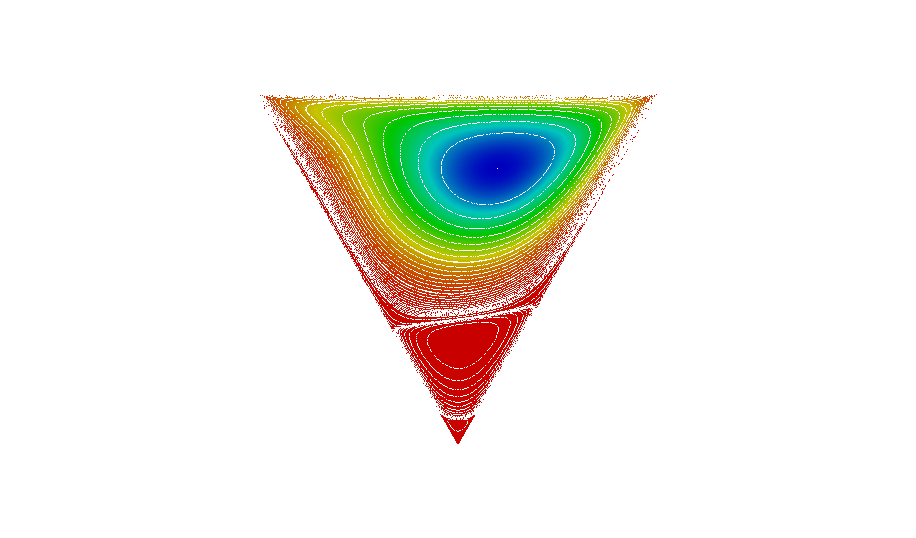
\includegraphics[scale=0.4, trim = 90mm 30mm 50mm 30mm, clip]{Equilateral_Re_100.png}
\caption{Re= 100}
\label{fig:2figsA}}
\qquad
\begin{minipage}{5cm}
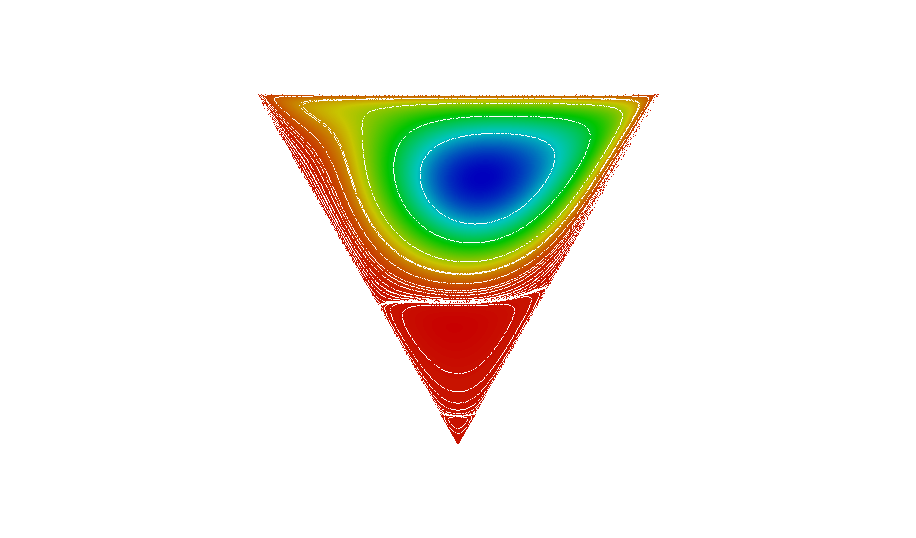
\includegraphics[scale=0.4, trim = 90mm 30mm 50mm 30mm, clip]{Equilateral_Re_200.png}
\caption{Re = 200}
%\label{fig:2figsB}
\end{minipage}
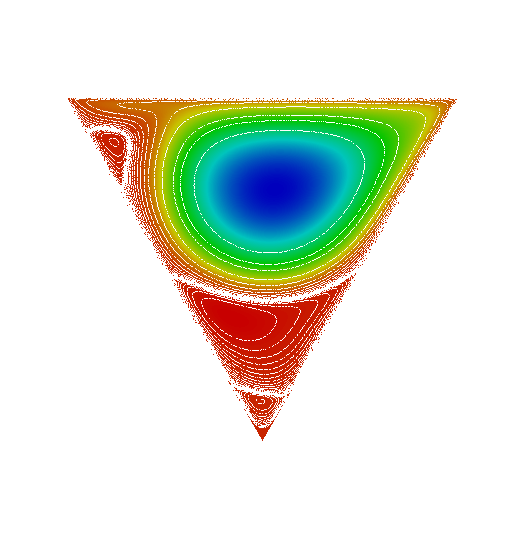
\includegraphics[scale=0.4]{Equilateral_Re_1000.png}
\caption{Re = 1000}
\caption{Streamfunctions of equilateral triangles} 
\end{figure}

Where the Reynolds number is defined as $Re = \frac{U}{\mu} $, where I set $U=1$ and controlled Re by changing $\mu$

Table~\ref{table:equilateral} looks at the position of the center eddy and the value of the streamfunction and vorticity at this point.

This study was done with 73541 vertices and 145664 cells. [1] used 131072 cells. The velocity was calculated in quadratic space.

We see that most of the streamfunction values, vorticity and position are similar to $10^{-2}$. As we increase Re the streamfunction value stays very similar, but the vorticity starts to become a little different but similar to $10^{-1}$. 
The position of the main eddy is very similar to Re = 1250, and changes a bit at Re = 1500.

\begin{table}[h]
  \centering%
  \begin{tabular}{l*{6}{c}r}
   & &Erturk and Gockol & & & Me\\
   \hline 
  Re & $\psi$ & $\omega$ &(x,y) & $\psi$ & $\omega$ & (x,y)  \\
  1   &   -0.2329  &-1.3788  & (0.0101, 04668) &-0.2329 & -1.3658  & (0.0109, 0.4617)  \\
  50   &  -0.2369 & -1.4689 & (0.3484, 04434)  & -0.2367 &-1.4708 & (0.3525, 0.4467)    \\
  100  & -0.2482 & -1.3669 & (0.3315, 0.3555)   & -0.2476 & -1.3599 &(0.3339, 0.3576)  \\
  200   & -0.2624 &-1.2518  & (0.2030, 0.2734)  & -0.2613 & -1.2459 & (0.1978, 0.2758 ) \\
  350   & -0.2724 & -1.1985 & (0.1556, 0.2383) &-0.2708 & -1.1887 & (0.1605, 0.2412)   \\
  500   & -0.2774 & -1.1791 &  (0.1319, 0.2207)  & -0.2754 &  -1.1666 & (0.1395, 0.2237)       \\
  750   &  -0.2818 & -1.1668 &  (0.1150, 0.2031) & -0.2793  & -1.1504  & (0.1160, 0.2056 ) \\
  1000   & -0.2844 & -1.1629 &(0.1116, 0.1973) & -0.2814  & -1.1427 & (0.1066, 0.1944) \\
  1250   & -0.2861 & -1.1624 & (0.1049, 0.1973) & -0.2826 & -1.1382 & (0.1066, 0.1944)   \\
  1500   & -0.2872 & -1.1639 & (0.1015, 0.1914)  & -0.2834 & -1.1354  & (0.1022, 0.1828)\\
  1750   &  -0.2881 & -1.1675 & (0.1015, 0.1914) & -0.2839 & -1.1336  & (0.1022, 0.1828)\\ 
\hline
\end{tabular}
  \caption{Eddies of equilateral Triangle}\label{table:equilateral}
\end{table}

\begin{table}[h]
  \centering%
  \begin{tabular}{l*{2}{c}r}
  Re &   $|\Delta \psi |$ &$|\Delta \omega |$  \\
  \hline 
  1   &  0.0   & $1.3*10^{-3}$\\
  50   & $2.0\cdot10^{-4}$ &$1.9*10^{-3}$    \\
  100  & $6.0*10^{-4}$ & $7.0*10^{-3}$ \\
  200   & $1.1*10^{-3}$ & $5.9*10^{-3}$ \\
  350   &  $ 1.6*10^{-3}$ &$9.8*10^{-3}$ \\
  500   &    $2.0*10^{-3}$   & $12.5*10^{-3}$\\
  750   &   $2.5*10^{-3}$ & $16.4*10^{-3}$\\
  1000   &  $3.0*10^{-3}$    & $20.2*10^{-3}$ \\
  1250   &   $3.5*10^{-3}$ & $24.2*10^{-3}$ \\
  1500   & $3.6*10^{-3}$  &$28.5*10^{-3}$ \\
  1750   &  $4.2*10^{-3}$ &$33.9*10^{-3}$\\ 
\hline
\end{tabular}
  \caption{ Absolute difference of $ \psi $ and $ \omega $ vs Erturk and Gockol}   
\end{table}

Next i studied what happens to the position of the main eddy when we refine the mesh. I used Re = 100 and matched the results with [1] (x,y) = (0.3315, 0.3555)

\begin{table}[h]
  \centering%
  \begin{tabular}{l*{6}{c}r}
   Vertices & $\Delta x$ & $\Delta y$ & (x,y) = (0.3315, 0.3555)\\
   \hline 
   273 & 0.052 & 0.067 & (0.3837, 0.4225) \\
   1064 & 0.070 & 0.01 &(0.4042, 0.3742)\\
   3946 & 0.042 & 0.008 & (0.3728, 0.3641)\\
   15134 & 0.0019 & 0.007 & (0.3515, 0.3633)\\
   59217 & 0.006 & 0.003 & (0.3375, 0.3594)\\
	\hline
 \end{tabular}
  \caption{Refinement study with Re = 100}
  \label{table:second eddy}
\end{table}

Next I considered an Isoceles Triangle with corner points: \newline
a = (-1, 0), b = (1, 0) ,c = (0, -4), with 64051 vertices and 126444 cells\newline
Again I looked at the position of the main eddy in Table~\ref{table:isoceles_triangle}.
Mesh:

\begin{figure}[h]
    \centering
    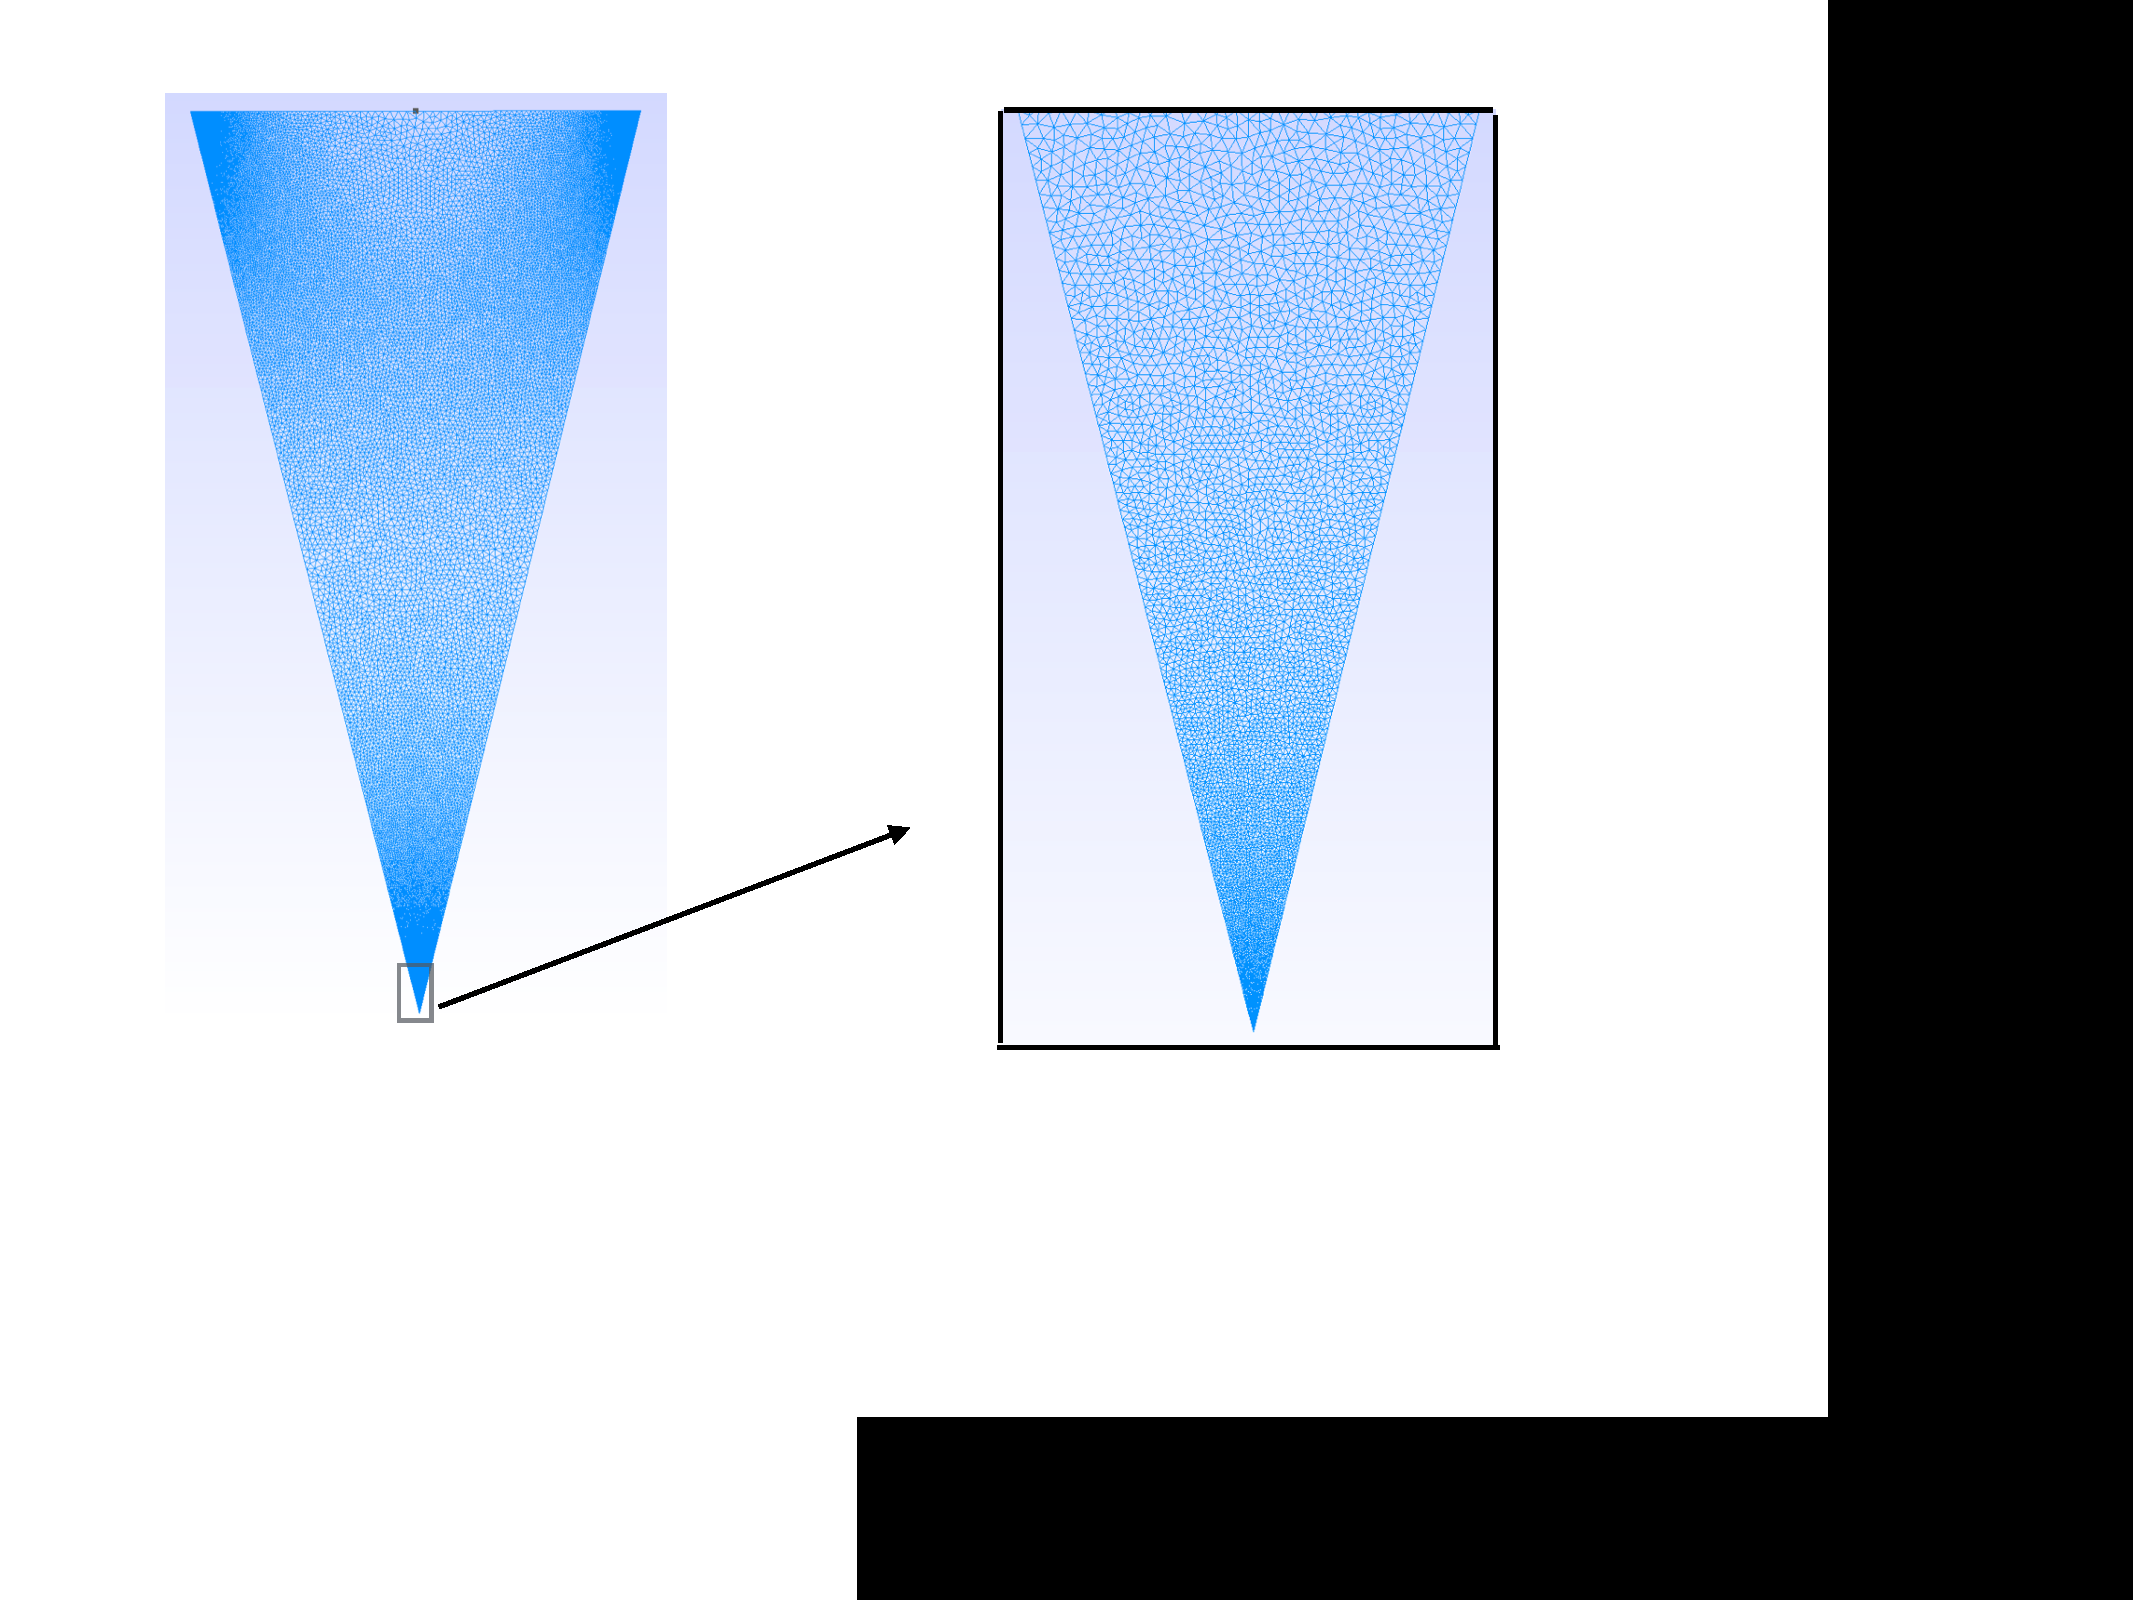
\includegraphics[trim = 30mm 50mm 30mm 10mm, clip, scale=0.6]{mesh_isoceles_pic.pdf}
    \caption{Mesh of isoceles triangle}
    \label{fig:yo}
\end{figure}


\begin{figure}
\centering
\parbox{5cm}{
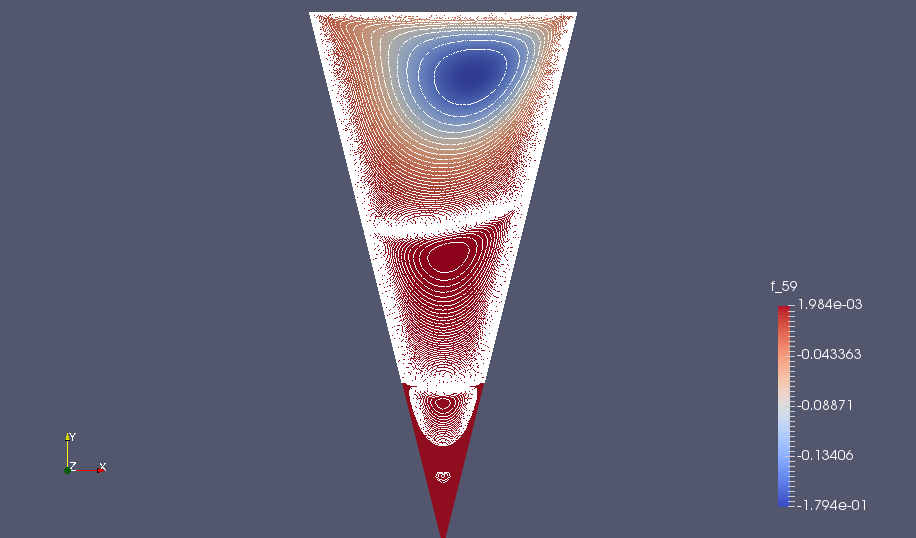
\includegraphics[scale=0.4, trim = 80mm 10mm 80mm 10mm, clip]{isoceles_Re_100.png}
\caption{Re= 100}
\label{fig:2figsA}}
\qquad
\begin{minipage}{5cm}
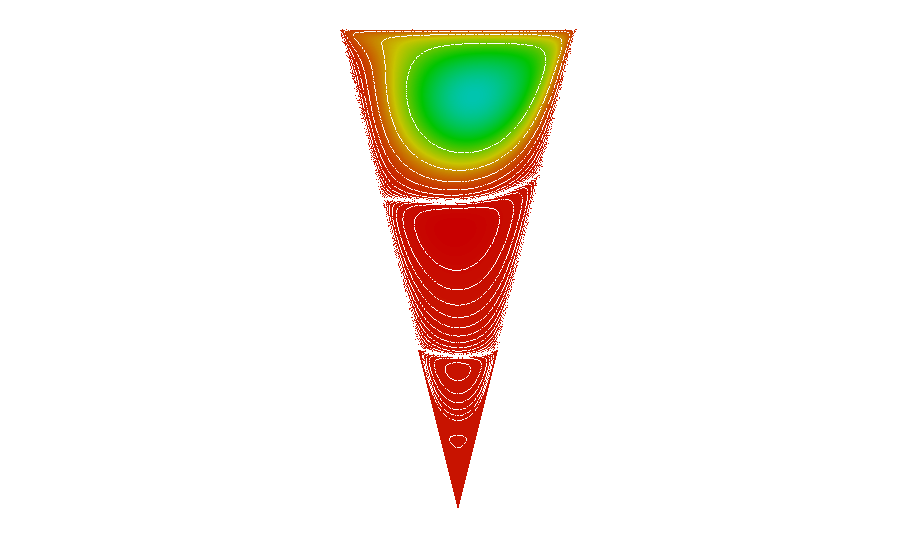
\includegraphics[scale= 0.4, trim = 80mm 10mm 80mm 10mm, clip]{isoceles_Re_200.png}
\caption{Re = 200}
\label{fig:2figsB}
\end{minipage}
\caption{Streamfunctions of isoceles triangles} 
\end{figure}

\begin{table}[h]
  \centering%
  \begin{tabular}{l*{6}{c}r}
   & Erturk and Gockol & Me\\
   \hline 
   Re &(x,y) & (x,y)  \\
   12.5 & (0.059, -0.391) & (0.0587, -0.4001 )\\ 
   25 & (0.115,-0.398) &  (0.1101, -0.3999 )\\
   100 & (0.213, -0.477)& (0.2124, -0.4767 ) \\
   200 & (0.129, -0.563)& (0.1275, -0.5608 )\\  
   \hline
  \end{tabular}
  \caption{Position of main eddy, isoceles triangle}\label{table:isoceles_triangle}
\end{table}

The next thing i looked at was where the second eddy was. This eddy is spinning the opposite direction so i had to look for the highest value of the stream function:

\begin{table}[h]
  \centering%
  \begin{tabular}{l*{6}{c}r}
   & Me\\
   \hline 
  	Re & $\psi$ & $\omega$& (x,y)   \\
	12.5 & 0.0002 & 0.0108 & (-0.0018, -2.1924)\\
	100 & 0.0020 & 0.0699  & (0.0490, -1.8199)\\
	200 &  0.0073 & 0.2183 & (-0.0237, -1.6809)\\
	\hline
 \end{tabular}
  \caption{Position of second eddy,isoceles }\label{table:second eddy}
\end{table}

As we see in figure 2 and 3 the second eddy moved up and to the left, which correlates with table 3.

The next thing i looked at was how many eddies i could find. According to [2] every eddy formed will be 406 times weaker then the previous. So the velocities and the very bottom eddies will be very small. To find these eddies I looked at the absolute velocities in the horizontal direction on a line straight through the mesh from the top at (0.0) to (0,-4). As we can see when the plot has a dip is where the velocities have changed direction and where we can find the eddies center. I used a very fine mesh at the bottom to catch as many eddies as a could. After a careful count, i got 9 eddies. This was done with Re=1, and with a mesh consisting of 57843 vertices and 113176 cells.

We can see that near the bottom we get disturbances.  As we see in Figure \ref{fig:2figsB} and ? that the mesh if very fine near the bottom corner. So the disturbances is probably caused by the fact that the computer can only represent numbers down to $10^{-17}$ [Ref].  One could argue that with a fine enough mesh and a computer able to represent infinitesimal numbers, that the number of eddies would go to infinity as we go down in the mesh.

If we compare to [2] in figure 5, where they have used a reynolds number of 0 (Stokes flow), we see that we get very similar results.


\begin{figure}[h]
    \centering
    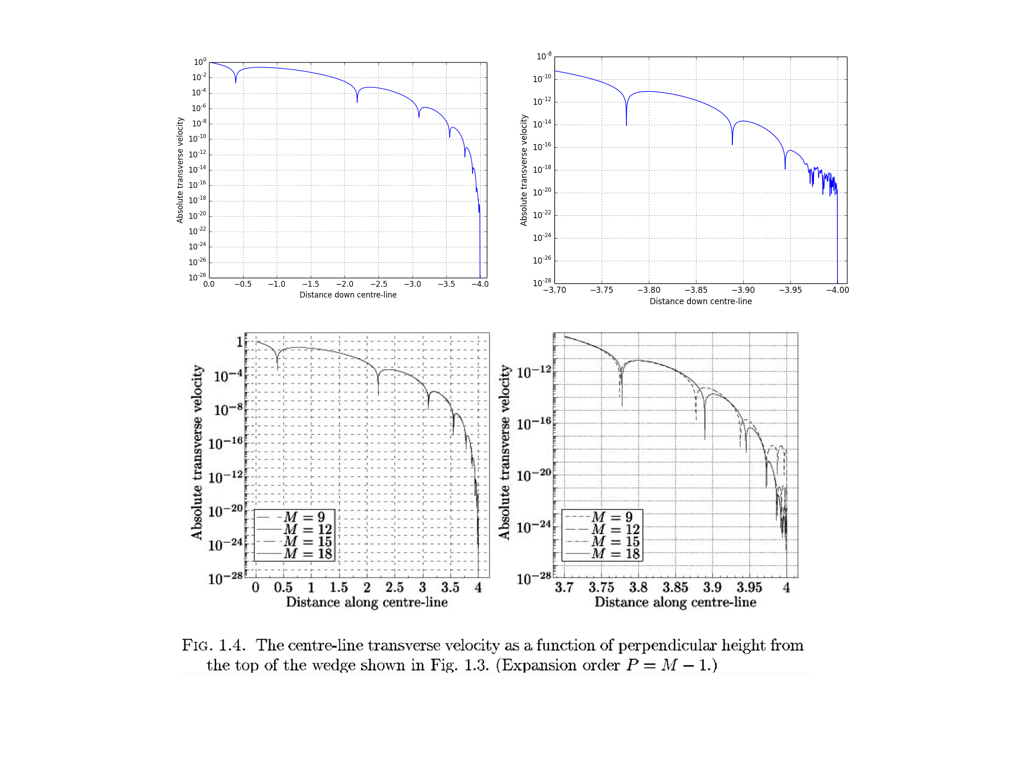
\includegraphics[trim = 50mm 20mm 0mm 20mm, clip, scale=0.5]{Eddy_plot_all.jpeg}
    \caption{Absolute transverse velocity, my study and }
    \label{fig:awesome_image}
\end{figure}

Representere tall i python, i pcen. ish 10e-18 eln.
Sjekke mat-inf komenpdiet 
Mulig at vi kan bestemme "steppet"
metode - lage meshet. steg for steg
POWERPOINT lage figurer, export i pdf
letter � lese tables

st�rre diff med h�yere Re . evnt

forfining av mesh med ett Re, med diff etc

diskutere mesh fra tidligere studier

vise hvor fint meshet er nederst. 


- Skru p� krylov l�ser for ett reynolds tall 

- G� fra LU l�ser til Krylov 

- Bilde av h�yere reynoldstall -- check

-  linear vs kvadratisk element  -- 

- bilde av mesh ved siden av hverandre

\bibliographystyle{vancouver}
\bibliography{bibliography}


%\begin{thebibliography}{9}

%\bibitem{lamport94}
 % Ercan Erturk and Orhan Gokcol,
%  \emph{Fine Grid Numerical Solutions of Triangular Cavity Flow},
 % The European Physical Journal - Applied Physics
%  2007.
%\bibitem{Erdos01} P. Erd\H os, \emph{Spectral hp Element Methods for CFD(Second Edition)}, Karniadakis, Sherwin, Oxford science publications, Oxford, 2005, pp. 11.

%\end{thebibliography}



\end{document}